%%%%%%%%%%%%%%%%%%%%%%%%%%%%%%%%%%%%%%%%%
% University/School Laboratory Report
% LaTeX Template
% Version 3.0 (4/2/13)
%
% This template has been downloaded from:
% http://www.LaTeXTemplates.com
%
% Original author:
% Linux and Unix Users Group at Virginia Tech Wiki
% (https://vtluug.org/wiki/Example_LaTeX_chem_lab_report)
%
% License:
% CC BY-NC-SA 3.0 (http://creativecommons.org/licenses/by-nc-sa/3.0/)
%
%%%%%%%%%%%%%%%%%%%%%%%%%%%%%%%%%%%%%%%%%

%----------------------------------------------------------------------------------------
%	PACKAGES AND DOCUMENT CONFIGURATIONS
%----------------------------------------------------------------------------------------

\documentclass[twocolumn]{article}

\usepackage{mhchem} % Package for chemical equation typesetting
\usepackage{siunitx} % Provides the \SI{}{} command for typesetting SI units
\usepackage{hyperref}
\usepackage{graphicx} % Required for the inclusion of images
\usepackage{tabularx}
\usepackage{float}
\usepackage{algorithm}
\usepackage{algpseudocode}
\usepackage{bm}
\usepackage{multirow}% http://ctan.org/pkg/multirow
\usepackage{hhline}% http://ctan.org/pkg/hhline


\setlength\parindent{0pt} % Removes all indentation from paragraphs

\renewcommand{\labelenumi}{\alph{enumi}.} % Make numbering in the enumerate environment by letter rather than number (e.g. section 6)

%\usepackage{times} % Uncomment to use the Times New Roman font

%----------------------------------------------------------------------------------------
%	DOCUMENT INFORMATION
%----------------------------------------------------------------------------------------

\title{UC Davis STA 242 2015 Spring Assignment 1} % Title
\author{Wenhao \textsc{Wu}, 9987583} % Author name
\date{\today} % Date for the report

\begin{document}
\maketitle % Insert the title, author and date

% If you wish to include an abstract, uncomment the lines below

\section{Data Parsing Procedure}
The basic data parsing procedure in our program is as follows.
\begin{enumerate}
    \item Check the legality of the file name.
    \item Call shell commend ``file'' and ``iconv'' to check and convert UTF-8
    files to ASCII files in order to avoid some UTF-8 symbols which may cause
    trouble to regular expression.
    \item use ``readLines'' to read in file.
    \item Locate the table head line using regular expression and estimate
    starting position and length of each field. If head line can not be found,
    this value should be specified manually.
    \item According to the field names specified in last step, generate a
    regular expression for one row in the data section and use it to locate the
    beginning and ending line of the data section.
    \item Use ``read.fwf'' (fixed-width method) to read the data into data
    frame.
\end{enumerate}
After parsing data into data frames, the data are then initially post-processed
with the following procedure.
\begin{enumerate}
    \item Expand the fields of each table with NA so that all table have the
    same 20 fiedls: ``place'', ``divtot'', ``name, ``number'', ``age'',
    ``hometown'', ``time\_gun'', ``time\_net'', ``pace'', ``seed'', ``split'',
    ``time\_five\_mile'', ``pace\_five\_mile'', ``time\_ten\_km'',
    ``pace\_ten\_km''.
    \item Decompose ``divtot'' field into ``div'' and 'tot'.
    \item Convert the name into lower case. If the name field contains
    ``unknown'' or ``unnamed'', set it to NA.
    \item Extract the USATF OPEN guideline or USATF Age-Group guidline
    indicator.
    \item Convert all time/pace/split domains into numeric (seconds).
    \item Convert the seed domain into logical.
    \item Process the hometown domain. This includes remove the wrong
    information from this field in case some one put their
    suite/apartment/street/email address or zipcode there. Then attempt to
    add three new fields to the table: ``hometown\_country'',
    ``hometown\_country'' and ``hometown\_city'', which are estimated on the
    best effort basis.
\end{enumerate}
Now the post processing is finished and we are ready to explore various aspect
of the data. The data, which are organized as a list of data frames.

\section{Interesting Findings}
The numbers of male and female runners taking part in the Cherry Blossom Run
from 1999 to 2010 are shown in Fig.~\ref{fig:num_runner}. Apparently, except
that there is a small decline from 1999 to 2000, the total number of both
male and female runners are increasing. Also, during the early years of Cherry
Blossom Run there are more male runners than female runners. However, the number
of female runners have suppassed that of the male runners starting from 2005 and
the gap have been increasing ever since.

\begin{figure}[h]
    \centering
    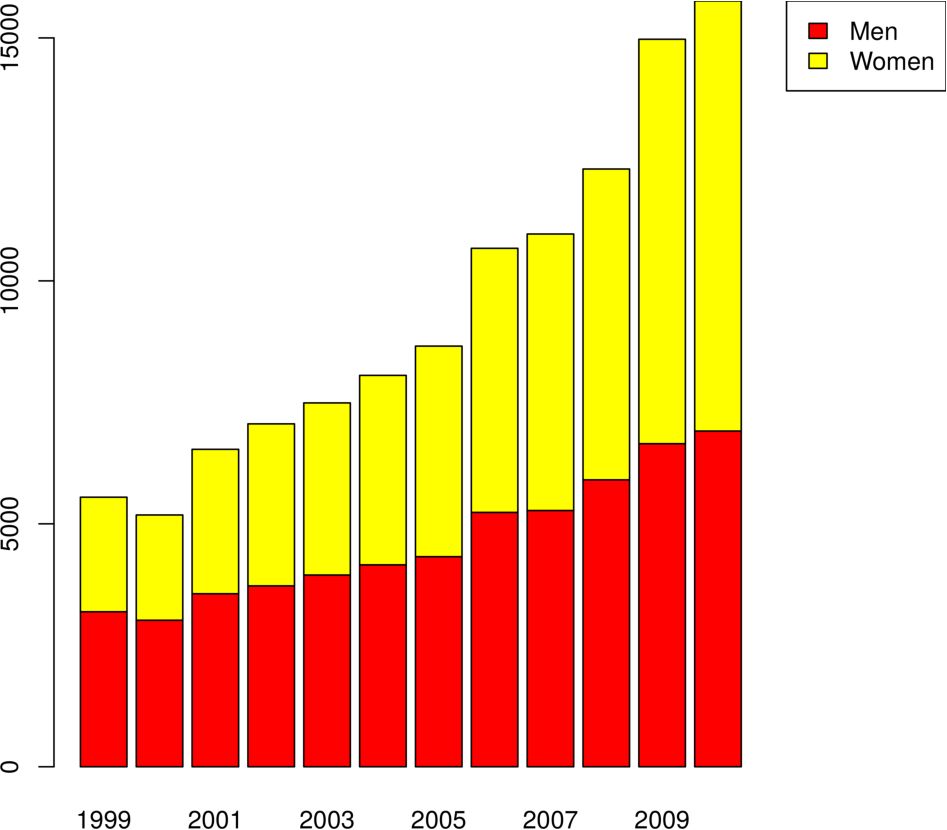
\includegraphics[width=2.5in]{figs/num_runner.pdf}
    \caption{The number of runners.}
    \label{fig:num_runner}
\end{figure}

Next we explore the performance of the runners in this event. In
Fig.~\ref{fig:time_net} we plot the average and the minimun net time (in
seconds) of the male and female runners. As we can see, the minimum net time for
men and women demonstrate a constant trend a little below and above 50 minutes,
respectively. However, the average net time shows a increasing trend, indicating
the average performance of the runners become worse and worse every year. This
is probably because that more and more non-pros are taking part in this run,
considering the fast increasing number of participants shown in
Fig.~\ref{fig:num_runner}.

\begin{figure}[h]
    \centering
    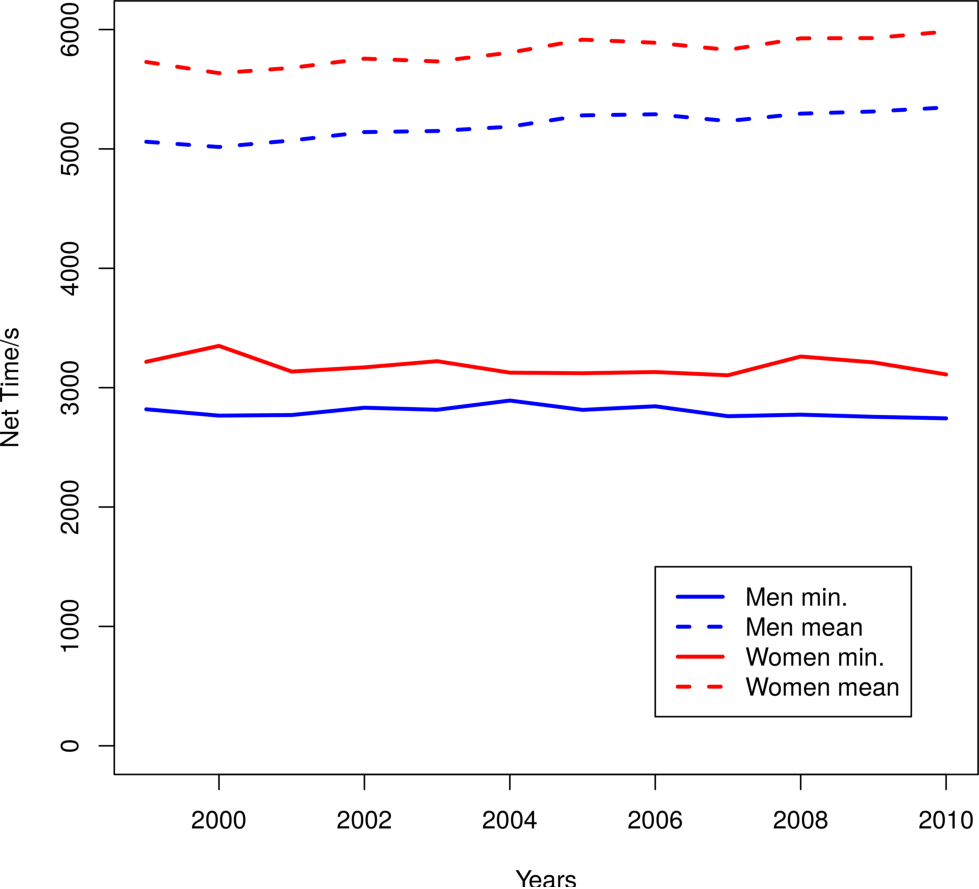
\includegraphics[width=2.5in]{figs/time_net.pdf}
    \caption{The average and minimum net time.}
    \label{fig:time_net}
\end{figure}

Now we focus on year 2010, when there are a total number of 15762 runners joined
this anual event. Among this runners, a majority of 15708 runners are identified
to be from US. In Fig.~\ref{fig:heatmap}, we plot the heatmap based on the
number of runners from different states. A majority of the runners are from
Maryland, Virginia and Washington D.C. There are also quite a few runners from
Pennsylvania and New York. This heatmap clearly shows that Cherry Blossom Run is
a popular local event.

\begin{figure}[h]
    \centering
    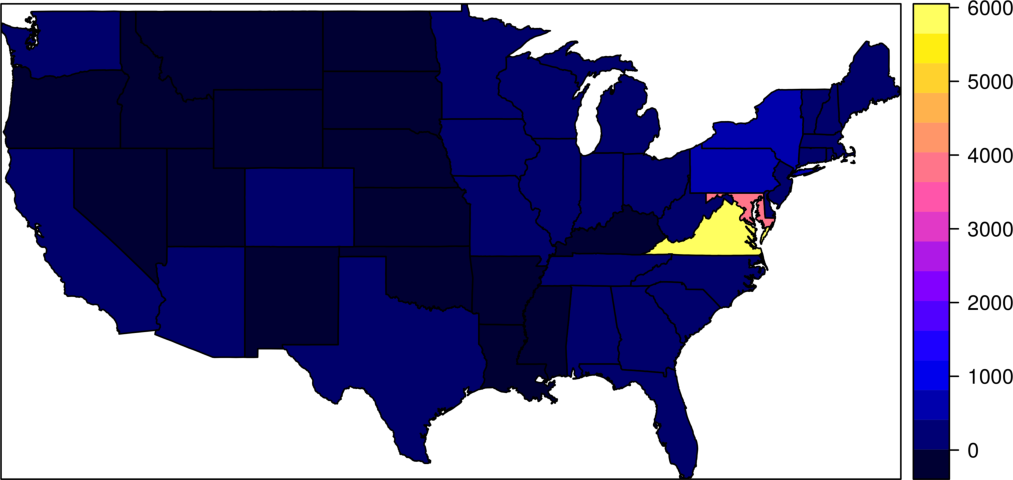
\includegraphics[width=3in]{figs/heatmap_usa_2010.pdf}
    \caption{The distributions of the runners across US.}
    \label{fig:heatmap}
\end{figure}

We have also looked at the age distribution of the male and female runners in
2010. Fig.~\ref{fig:age_male} and Fig.~\ref{fig:age_female} show the recorded
age ranges of each age group and the density w.r.t age in that group (so that
the size of each column represent the total number of runners in the
corresponding group). We notice that the youngest runners are 11 years old
and there is a senior runners at the age of 86 (holy!). The largest age group
for both women and men are both the one from 25 to 29.

\begin{figure}[h]
    \centering
    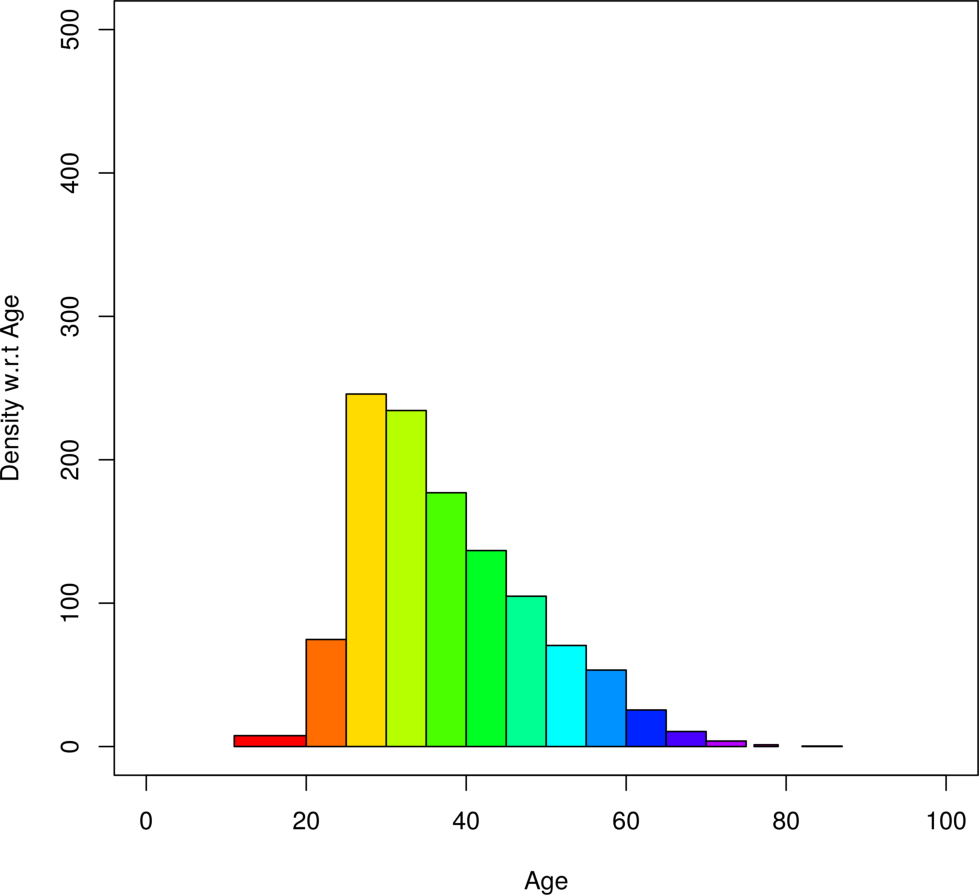
\includegraphics[width=2.5in]{figs/group_m2010.pdf}
    \caption{Age distribution of male runners in 2010.}
    \label{fig:age_male}
\end{figure}

\begin{figure}[h]
    \centering
    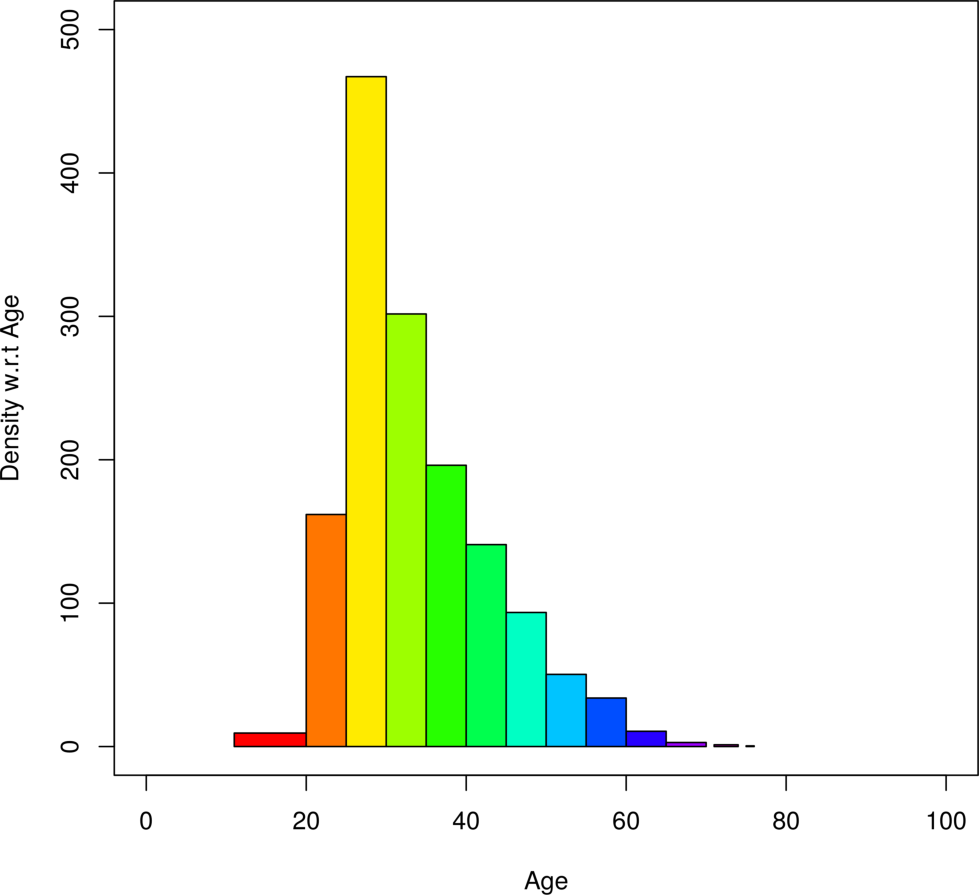
\includegraphics[width=2.5in]{figs/group_f2010.pdf}
    \caption{Age distribution of female runners in 2010.}
    \label{fig:age_female}
\end{figure}

It is also interesting relate the performance of the runners with their ages. In
Fig.~\ref{fig:time_group_age}, we plot the mean and minimum net time within each
age group. Considering the minimum net time, we notice that the best
performance is reached by runners from 20 to 24. Considering the mean net time,
the average performance is getting worse and worse as the age grows. However,
age group 40-44 shows a better performance than age group 35-39 in both the mean
and min net time for both men and women.

\begin{figure}[!h]
    \centering
    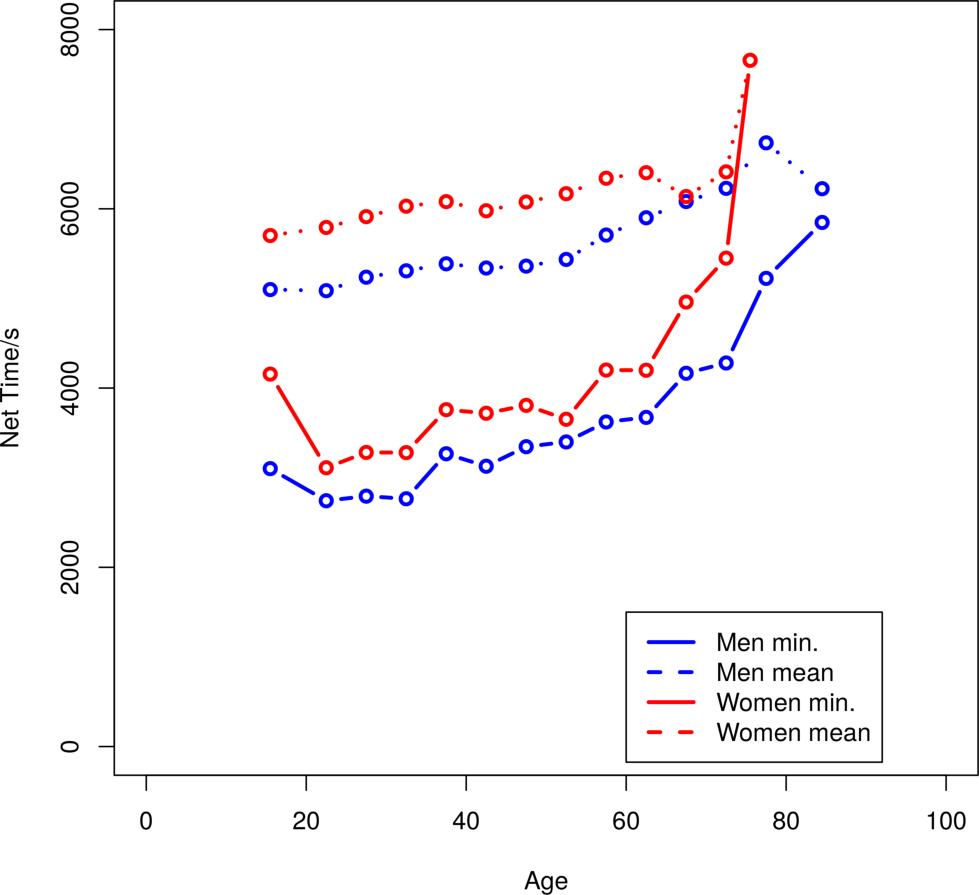
\includegraphics[width=2.5in]{figs/time_net_group_2010.pdf}
    \caption{Mean and minimum net time versus age group.}
    \label{fig:time_group_age}
\end{figure}

Finally, we try to found all records for one individual runner across different
years based on one piece of record in one year. To do so, we adopt a very
simple rule: we assume that the name and gender (no offense) of each individual
do not change across years. Also we assume that by the time of Cherry Blossom
Run, the age of each individual will increase by 1 each year. As an example, we
consider Christopher Dean, who got 38 place in 2003.
All 4 pieces of record matched to it are listed in Table~\ref{tab:match}. As we
can see, this guy took part in this event from 2003 to 2006 in a row, achieved
his best place in 2005. Also the number on Chris's shirt is different every
year. This simple mapping scheme works well for some one with neat records
across different files. However, it is limited in the aspect that
\begin{itemize}
    \item If the age field is NA this would not work. Perhaps we could also try
    combining the hometown information.
    \item Although we performed a few cleanning steps for the name field, it is
    still possible that the same person have names that can not be perfectly
    matched accross different files. This might happen when someone mis-spelled
    his name, when there is an AKA in the middle of the name, when the first and
    last name got reverted or when a female runner get married. This problem
    might be alleviated with the approximated string match method from
    package `stringdist` by allowing non-perfect match of
    the name field.
\end{itemize}

\begin{table*}[!h]
    \renewcommand{\arraystretch}{1.3}
    \caption{All records of Christopher Dean found in different files.}
    \label{tab:match}
    \centering
    \begin{tabular}{c|ccccccccc}
        \hline
        year & place & div/tot & number & age & hometown & time gun &
        time net & pace & seed \\
        \hline
        2003 & 38 & 38/1999  & 2466 & 28 & Alexandria VA &
        3316 & 3314 & NA & NA\\
        2004 & 48 & 39/2242 & 7328 & 29 & Alexandria VA & 3378 & 3377 & NA & NA
        \\
        2005 & 33 & 32/2290 & NA & 30 & Alexandria VA & 3312 & 3312 & 332 & NA
        \\
        2006 & 120 & 91/2892 & 4652 & 31 & Alexandria & 3655 & 3652 & 366 &
        FALSE \\
        \hline
    \end{tabular}
\end{table*}
%\pagebreak
%	BIBLIOGRAPHY
%----------------------------------------------------------------------------------------

%\bibliographystyle{unsrt}
%\bibliography{myrefs}

%----------------------------------------------------------------------------------------


\end{document}